% ------------------------------------------------
% PROFESSIONAL PROJECT BLUEPRINT TEMPLATE
% ------------------------------------------------
\documentclass[12pt,a4paper]{report}

% -------------------------------
% PACKAGES
% -------------------------------
\usepackage[utf8]{inputenc}
\usepackage[T1]{fontenc}
\usepackage{lmodern}
\usepackage{geometry}
\geometry{margin=1in}
\usepackage{setspace}
\onehalfspacing
\usepackage{graphicx}
\usepackage{fancyhdr}
\usepackage{titlesec}
\usepackage{hyperref}
\usepackage{tocloft}
\usepackage{xcolor}
\usepackage{tikz}            % For the colored background on title page
\usepackage{lipsum}          % Sample text (remove later)

% -------------------------------
% COLORS
% -------------------------------
\definecolor{myblue}{HTML}{0B3D91}   % Deep corporate blue
\definecolor{lightgray}{HTML}{F5F5F5}
\definecolor{darkgray}{HTML}{2E2E2E}

% -------------------------------
% LINK STYLES
% -------------------------------
\hypersetup{
    colorlinks=true,
    linkcolor=myblue,
    urlcolor=myblue,
    citecolor=myblue
}

% -------------------------------
% HEADER & FOOTER
% -------------------------------
\pagestyle{fancy}
\fancyhf{}
\fancyhead[L]{\textbf{Project Blueprint}}
\fancyhead[R]{\leftmark}
\fancyfoot[C]{\thepage}
\renewcommand{\headrulewidth}{0.4pt}
\renewcommand{\footrulewidth}{0.4pt}

% -------------------------------
% SECTION STYLE
% -------------------------------
\titleformat{\chapter}[hang]{\bfseries\Huge\color{myblue}}{\thechapter\quad}{0pt}{}
\titleformat{\section}[hang]{\bfseries\Large\color{myblue}}{\thesection\quad}{0pt}{}
\titleformat{\subsection}[hang]{\bfseries\large\color{myblue}}{\thesubsection\quad}{0pt}{}

% -------------------------------
% PANDOC COMMANDS
% -------------------------------
% ------------------------------------------------
% Pandoc LaTeX Compatibility Definitions
% ------------------------------------------------
% This file defines helper macros and package imports
% commonly used by Pandoc-generated LaTeX files.

% ---------- Required Packages ----------
\usepackage{longtable}    % For multi-page tables
\usepackage{booktabs}     % For \toprule, \midrule, \bottomrule
\usepackage{array}        % Better table column handling
\usepackage{calc}         % For table width calculations
\usepackage{etoolbox}     % For \AtBeginEnvironment, etc.
\usepackage{amssymb}      % For symbols like \square

% ---------- Pandoc Helper Commands ----------
% Used in Pandoc-generated itemize lists
\providecommand{\tightlist}{%
  \setlength{\itemsep}{0pt}\setlength{\parskip}{0pt}}

% For inline subscripts created from Markdown (e.g., ~text~)
\providecommand{\textsubscript}[1]{\ensuremath{_{\text{#1}}}}

% For passthrough raw LaTeX (rare but harmless)
\providecommand{\passthrough}[1]{#1}

% ---------- Optional: Style Tweak ----------
% Add spacing above/below longtables for readability
\AtBeginEnvironment{longtable}{\setlength{\LTpre}{0.5em}\setlength{\LTpost}{0.5em}}

% ---------- Optional: Square Checkbox Symbol ----------
% If your Markdown uses "[$\square$]" for checklists
% Already available from amssymb, so no extra definition needed.

% ---------- Notes ----------
% This file ensures Pandoc .tex snippets work smoothly
% when included into your main LaTeX project.
% Include it in your preamble:
%   % ------------------------------------------------
% Pandoc LaTeX Compatibility Definitions
% ------------------------------------------------
% This file defines helper macros and package imports
% commonly used by Pandoc-generated LaTeX files.

% ---------- Required Packages ----------
\usepackage{longtable}    % For multi-page tables
\usepackage{booktabs}     % For \toprule, \midrule, \bottomrule
\usepackage{array}        % Better table column handling
\usepackage{calc}         % For table width calculations
\usepackage{etoolbox}     % For \AtBeginEnvironment, etc.
\usepackage{amssymb}      % For symbols like \square

% ---------- Pandoc Helper Commands ----------
% Used in Pandoc-generated itemize lists
\providecommand{\tightlist}{%
  \setlength{\itemsep}{0pt}\setlength{\parskip}{0pt}}

% For inline subscripts created from Markdown (e.g., ~text~)
\providecommand{\textsubscript}[1]{\ensuremath{_{\text{#1}}}}

% For passthrough raw LaTeX (rare but harmless)
\providecommand{\passthrough}[1]{#1}

% ---------- Optional: Style Tweak ----------
% Add spacing above/below longtables for readability
\AtBeginEnvironment{longtable}{\setlength{\LTpre}{0.5em}\setlength{\LTpost}{0.5em}}

% ---------- Optional: Square Checkbox Symbol ----------
% If your Markdown uses "[$\square$]" for checklists
% Already available from amssymb, so no extra definition needed.

% ---------- Notes ----------
% This file ensures Pandoc .tex snippets work smoothly
% when included into your main LaTeX project.
% Include it in your preamble:
%   % ------------------------------------------------
% Pandoc LaTeX Compatibility Definitions
% ------------------------------------------------
% This file defines helper macros and package imports
% commonly used by Pandoc-generated LaTeX files.

% ---------- Required Packages ----------
\usepackage{longtable}    % For multi-page tables
\usepackage{booktabs}     % For \toprule, \midrule, \bottomrule
\usepackage{array}        % Better table column handling
\usepackage{calc}         % For table width calculations
\usepackage{etoolbox}     % For \AtBeginEnvironment, etc.
\usepackage{amssymb}      % For symbols like \square

% ---------- Pandoc Helper Commands ----------
% Used in Pandoc-generated itemize lists
\providecommand{\tightlist}{%
  \setlength{\itemsep}{0pt}\setlength{\parskip}{0pt}}

% For inline subscripts created from Markdown (e.g., ~text~)
\providecommand{\textsubscript}[1]{\ensuremath{_{\text{#1}}}}

% For passthrough raw LaTeX (rare but harmless)
\providecommand{\passthrough}[1]{#1}

% ---------- Optional: Style Tweak ----------
% Add spacing above/below longtables for readability
\AtBeginEnvironment{longtable}{\setlength{\LTpre}{0.5em}\setlength{\LTpost}{0.5em}}

% ---------- Optional: Square Checkbox Symbol ----------
% If your Markdown uses "[$\square$]" for checklists
% Already available from amssymb, so no extra definition needed.

% ---------- Notes ----------
% This file ensures Pandoc .tex snippets work smoothly
% when included into your main LaTeX project.
% Include it in your preamble:
%   \input{pandoc-compat.tex}




% -------------------------------
% TITLE PAGE (CUSTOM DESIGN)
% -------------------------------
\newcommand{\makemytitle}{
\begin{titlepage}
    \begin{tikzpicture}[remember picture,overlay]
        % Background rectangle (change 'myblue' to 'darkgray' for a gray version)
        \fill[darkgray] (current page.south west) rectangle (current page.north east);
    \end{tikzpicture}

    \vspace*{3cm}
    \begin{center}
        \includegraphics[width=0.25\textwidth]{../../Assets/Main_logo.png} \\[2cm] % Replace with your logo file

        {\Huge\bfseries\color{white} Project Blueprint}\\[0.5cm]
        {\Large\color{white} IT in a real organization}\\[2cm]

        {\large\color{white} André Martins, Manon, Elvin, Leonardo Coimbra and Tomás Coimbra}\\[0.2cm]
        {\color{white} Lamtco Solutions}\\[0.2cm]
        {\color{white}\href{mailto:0230991223@uni.lu}{0230991223@uni.lu}}\\[2cm]

        {\large\color{white}\today}
    \end{center}
\end{titlepage}
}

% -------------------------------
% DOCUMENT START
% -------------------------------
\begin{document}

% Custom Cover Page
\makemytitle
\thispagestyle{empty}
\clearpage

% Table of Contents
\pagenumbering{roman}
\tableofcontents
\clearpage

% Main Content
\pagenumbering{arabic}

\chapter{Introduction}

In this document you will find the main definition of have this project. You will find the Specification definition as well as the main system design.
There will also be a section dedicated to the current system's risks.

\chapter{Specification}

The Specification has been defined in three different levels: \textbf{Epics, User stories and use cases}. You will now find in the following pages the project specification in the tree levels.

\section{Epics}

\subsection{Epic: User system}\label{epic-user-system}

\textbf{Epic ID:} EPIC-1 \textbf{Status:} \texttt{Proposed}
\textbf{Priority:} \texttt{High} \\
\textbf{Theme:} Connecting all the users (employees) to the app
infrastructure

\textbf{Created:} 15/10/2025 \textbf{Last Updated:} 15/10/2025\\
\textbf{Target Release:} 08/12/2025

\subsubsection{Epic Overview}\label{epic-overview}

\textbf{Business Problem:}

Currently managing working hours always requires each employee to have
additional hardware (badge system, need of a computer, \ldots) or they
still write all their working hours in a paper format.

In order to solve this issue, he have decided to implement a mobile
application software that would allow us all employees to use their
personal phones in order to book all their working hours.

\textbf{Business Value:}

The software eliminates the need for additional hardware and digitalizes
the entry of working hours, improving efficiency and avoiding trickery.

\textbf{Success Metrics:} - Metric 1: Being able to add hours into the
system by no more that 5 button actions - Metric 2: Support all
platforms - Metric 3: {[}Still to continue{]}

\subsubsection{Scope}\label{scope}

\paragraph{In Scope\\}\label{in-scope}

\begin{itemize}
\tightlist
\item
  Build an intuitive, easy-to-use mobile application
\item
  Send localization and timings of the user to the data server
\item
  Make attractive design for employees
\end{itemize}

\paragraph{Out of Scope\\}\label{out-of-scope}

\begin{itemize}
\tightlist
\item
  Application integrated into company car software
\item
  Fully automated service (by entering a certain location with your
  device)
\end{itemize}

\subsubsection{User Personas}\label{user-personas}

\begin{itemize}
\tightlist
\item
  \textbf{Employee User:} Enters the start/end of their shift.
\end{itemize}

\subsubsection{User Stories}\label{user-stories}

\begin{longtable}[]{@{}llll@{}}
\toprule\noalign{}
Story ID & Story Title & Status & Priority \\
\midrule\noalign{}
\endhead
\bottomrule\noalign{}
\endlastfoot
{[}US-1{]} & Employer Shift Monitoring & \texttt{Backlog} &
\texttt{Low} \\
{[}US-2{]} & Employee Shift Punch-in (Start Shift) & \texttt{Backlog} &
\texttt{High} \\
{[}US-3{]} & Employee Shift Punch-out (End Shift) & \texttt{Backlog} &
\texttt{High} \\
{[}US-4{]} & Employee Reminders & \texttt{Backlog} & \texttt{Low} \\
\end{longtable}

% \subsection{Technical Considerations}\label{technical-considerations}

% \textbf{Architecture Impact:} - {[}How this affects system
% architecture{]} - {[}New components/services required{]}

% \textbf{Dependencies:} - {[}External systems/dependencies{]} - {[}Other
% epics/teams we depend on{]}

% \textbf{Risks \& Mitigations:} - \textbf{{[}Risk 1{]}:}
% {[}Description{]} - {[}Mitigation strategy{]} - \textbf{{[}Risk 2{]}:}
% {[}Description{]} - {[}Mitigation strategy{]}

% \textbf{Non-Functional Requirements:} - \textbf{Performance:} {[}e.g.,
% Response time under 2 seconds{]} - \textbf{Security:} {[}e.g.,
% Role-based access control{]} - \textbf{Scalability:} {[}e.g., Support X
% concurrent users{]} - \textbf{Reliability:} {[}e.g., 99.9\% uptime{]}

% \subsection{Definition of Ready}\label{definition-of-ready}

% \begin{itemize}
% \tightlist
% \item[$\square$]
%   Business value clearly defined
% \item[$\square$]
%   Success metrics established
% \item[$\square$]
%   High-level scope approved
% \item[$\square$]
%   User stories identified and estimated
% \item[$\square$]
%   Technical dependencies resolved
% \item[$\square$]
%   UX/design completed (if applicable)
% \end{itemize}

% \subsection{Definition of Done}\label{definition-of-done}

% \begin{itemize}
% \tightlist
% \item[$\square$]
%   All user stories completed and accepted
% \item[$\square$]
%   Success metrics validated
% \item[$\square$]
%   Documentation updated
% \item[$\square$]
%   Integration tests passing
% \item[$\square$]
%   Performance requirements met
% \item[$\square$]
%   Deployed to production
% \item[$\square$]
%   Business stakeholders signed off
% \end{itemize}

% \subsection{Open Questions}\label{open-questions}

% \begin{itemize}
% \tightlist
% \item
%   {[}Question 1{]}
% \item
%   {[}Question 2{]}
% \item
%   {[}Assumptions we're making{]}
% \end{itemize}

% \subsection{Related Artifacts}\label{related-artifacts}

% \begin{itemize}
% \tightlist
% \item
%   {[}Links to wireframes, technical designs, research, etc.{]}
% \end{itemize}

{
    \let\section\subsection
    \let\subsection\subsubsection
    \let\subsubsection\paragraph

    \section{Epic: Timelink Admin
Platform}\label{epic-timelink-admin-platform}

\textbf{Epic ID:} EPIC-002 \textbf{Status:} \texttt{Proposed}
\textbf{Priority:} \texttt{High} \textbf{Theme:} Helping managers and
CEO's manage the working hours of their employees

\textbf{Created:} 15/10/2025 \textbf{Last Updated:} 16/10/2025
\textbf{Target Release:} 08/12/2025

% \begin{center}\rule{0.5\linewidth}{0.5pt}\end{center}

\subsection{Epic Overview}\label{epic-overview}

\textbf{Business Problem:} Currently all managers do quite struggle to
manage and monitor the working hours of their workers and working places
respectively. It is really easy to make lose the amount of labor that
has been relaised in a working place or individual in live and in an
easy way.

\textbf{Business Value:} The Admin Platform helps companies save time
and reduce errors by showing all information in one clear system. It
makes it easier to see all the data represented in several graphical
representations.

\textbf{Success Metrics:} - Reduce manual work for administrators by at
least 60\% - 100\% synchronization between Admin Platform and Data
Server - Reach 95\% user satisfaction in the first release - System
uptime above 99.9\% during testing

% \begin{center}\rule{0.5\linewidth}{0.5pt}\end{center}

\subsection{Scope}\label{scope}

\subsubsection{In Scope}\label{in-scope}

\begin{itemize}
\tightlist
\item
  Build a web-based Admin Platform using React Native
\item
  Connect the Admin Platform to the main Data Server (Spring Boot / SQL)
\item
  Create login and role-based access (admin users only)
\item
  Add dashboards with tables and graphs for all the employee data
\item
  Allow basic CRUD functions (create, read, update, delete) for all
  employee data
\end{itemize}

\subsubsection{Out of Scope}\label{out-of-scope}

\begin{itemize}
\tightlist
\item
  Full integration with external systems (like GPS tracking)
\item
  Data export in XML or other formats
\item
  Mobile version for admin users (web only for now)
\end{itemize}

% \begin{center}\rule{0.5\linewidth}{0.5pt}\end{center}

\subsection{User Personas}\label{user-personas}

\begin{itemize}
\tightlist
\item
  \textbf{Admin User:} Works in HR or management. Needs to see and
  manage all employee data, hours, and working places quickly.
\item
  \textbf{Company Manager:} Supervises multiple workplaces and wants to
  be able to easily review statistics and reports.
\end{itemize}

% \begin{center}\rule{0.5\linewidth}{0.5pt}\end{center}

\subsection{User Stories}\label{user-stories}

\begin{longtable}[]{@{}
  >{\raggedright\arraybackslash}p{(\linewidth - 6\tabcolsep) * \real{0.2381}}
  >{\raggedright\arraybackslash}p{(\linewidth - 6\tabcolsep) * \real{0.3095}}
  >{\raggedright\arraybackslash}p{(\linewidth - 6\tabcolsep) * \real{0.2143}}
  >{\raggedright\arraybackslash}p{(\linewidth - 6\tabcolsep) * \real{0.2381}}@{}}
\toprule\noalign{}
\begin{minipage}[b]{\linewidth}\raggedright
Story ID
\end{minipage} & \begin{minipage}[b]{\linewidth}\raggedright
Story Title
\end{minipage} & \begin{minipage}[b]{\linewidth}\raggedright
Status
\end{minipage} & \begin{minipage}[b]{\linewidth}\raggedright
Priority
\end{minipage} \\
\midrule\noalign{}
\endhead
\bottomrule\noalign{}
\endlastfoot
US-5 & As an admin, I want to log in securely to the Admin Platform &
\texttt{Backlog} & \texttt{High} \\
US-6 & As an admin, I want to view employee working hours and working
places & \texttt{Backlog} & \texttt{High} \\
US-7 & As an admin, I want to see graphs of total hours worked per
working place & \texttt{Backlog} & \texttt{Medium} \\
US-8 & As an admin, I want to add and remove users from the system &
\texttt{Backlog} & \texttt{Medium} \\
US-9 & As an admin, I want to see connection status with the Data Server
& \texttt{Backlog} & \texttt{Low} \\
US-10 & As an admin, I want to filter employee data by department or
project, so that I can analyze work distribution more efficiently &
\texttt{Backlog} & \texttt{Medium} \\
US-11 & As an admin, I want to edit working places and assign employees
to them, so that I can maintain an up-to-date organizational structure &
\texttt{Backlog} & \texttt{High} \\
US-12 & As an admin, I want to view an activity log of recent changes in
the system, so that I can track who modified what and when &
\texttt{Backlog} & \texttt{Medium} \\
\end{longtable}

% \begin{center}\rule{0.5\linewidth}{0.5pt}\end{center}

\subsection{Technical Considerations}\label{technical-considerations}

\textbf{Architecture Impact:} - The Admin Platform will communicate
directly with the Data Server using a REST Controller. - Requires a new
web frontend built with React Native for Web. - Backend data comes from
the existing Spring Boot server with SQL database.

\textbf{Dependencies:} - Data Server must be ready before Admin Platform
API integration.

\textbf{Risks \& Mitigations:} - \textbf{Risk 1:} Admin Platform may
load slowly with big data sets -- \emph{Mitigation:} Optimize queries. -
\textbf{Risk 2:} Inconsistent data between server and UI --
\emph{Mitigation:} Add sync checks and server-side validation.

\textbf{Non-Functional Requirements:}\\
- \textbf{Performance:} Pages should load in under 2 seconds. -
\textbf{Security:} Only authorized admin users can log in. -
\textbf{Scalability:} Should support up to 100 admin users per company.
- \textbf{Reliability:} 99.9\% uptime expected in testing phase.

\begin{center}\rule{0.5\linewidth}{0.5pt}\end{center}

% \subsection{Definition of Ready}\label{definition-of-ready}

% \begin{itemize}
% \tightlist
% \item[$\boxtimes$]
%   Business value clearly defined
% \item[$\boxtimes$]
%   Success metrics established
% \item[$\boxtimes$]
%   High-level scope approved
% \item[$\boxtimes$]
%   User stories identified and estimated
% \item[$\square$]
%   Technical dependencies resolved
% \item[$\square$]
%   UX/design completed (not started yet)
% \end{itemize}

% \begin{center}\rule{0.5\linewidth}{0.5pt}\end{center}

% \subsection{Definition of Done}\label{definition-of-done}

% \begin{itemize}
% \tightlist
% \item[$\square$]
%   All user stories completed and accepted
% \item[$\square$]
%   Success metrics validated
% \item[$\square$]
%   Documentation updated
% \item[$\square$]
%   Integration tests passing
% \item[$\square$]
%   Performance requirements met
% \item[$\square$]
%   Deployed to production
% \item[$\square$]
%   Business stakeholders signed off
% \end{itemize}

% \begin{center}\rule{0.5\linewidth}{0.5pt}\end{center}

% \subsection{Open Questions}\label{open-questions}

% \begin{itemize}
% \tightlist
% \item
%   Is multi-language support required for version 1?
% \end{itemize}

% \begin{center}\rule{0.5\linewidth}{0.5pt}\end{center}

% \subsection{Related Artifacts}\label{related-artifacts}

% \begin{itemize}
% \tightlist
% \item
%   {[}Links to wireframes, technical designs, research, etc.{]}
% \end{itemize}

}

\section{User Stories}

{
    \let\section\subsection
    \let\subsection\subsubsection
    \let\subsubsection\paragraph

    \section{User Story 01}\label{user-story-01}

\subsection{Epic: EPIC-01}\label{epic-epic-01}

\subsubsection{01: Employer Shift
Monitoring}\label{employer-shift-monitoring}

\textbf{Status:} \texttt{Backlog}

\textbf{As a(n)} Employee,\\
\textbf{I want to} see a list of all my logged hours,\\
\textbf{So that} I can monitor attendance and verify shift compliance.

\textbf{Acceptance Criteria:} - {[} {]} Show weekly, monthly, or yearly
totals per employee. - {[} {]} Show hours in graphical diagram (example:
histogram). - {[} {]} View detailed employee information (site, total
hours, employee since, etc.).

\textbf{Technical Notes:} - Graphical Diagrams could be generated at the
end of each week.

\textbf{Estimate:} 2-3 Story Points \textbf{Priority:} \texttt{Low}

    \section{User Story 02}\label{user-story-02}

\subsection{Epic: EPIC-01}\label{epic-epic-01}

\subsubsection{02: Employee Shift Punch-in (Start
Shift)}\label{employee-shift-punch-in-start-shift}

\textbf{Status:} \texttt{Backlog}

\textbf{As a(n)} Employee,\\
\textbf{I want to} start my shift by pressing a ``Start Shift'' button
in the application,\\
\textbf{So that} the system may begin logging my working hours
accurately.

\textbf{Acceptance Criteria:} - {[} {]} The application prompts a
confirmation before starting a shift. - {[} {]} Access the ``Start
Shift'' button within 3 taps or fewer from opening application. - {[}
{]} The application indicates clearly that a shift has started.

\textbf{Technical Notes:} - Button sizes should be considerably large to
take gloves and thicker fingers into consideration.

\textbf{Estimate:} 2 Story Points \textbf{Priority:} \texttt{High}

    \section{User Story 03}\label{user-story-03}

\subsection{Epic: EPIC-01}\label{epic-epic-01}

\subsubsection{03: Employee Shift Punch-out (End
Shift)}\label{employee-shift-punch-out-end-shift}

\textbf{Status:} \texttt{Backlog}

\textbf{As a(n)} Employee,\\
\textbf{I want to} end my shift by pressing a ``End Shift'' button in
the application,\\
\textbf{So that} the system may log the end of my shift accurately.

\textbf{Acceptance Criteria:} - {[} {]} The app prompts a confirmation
before ending a shift. - {[} {]} Getting to ``End Shift'' button should
take no more than 3 clicks. - {[} {]} The application indicates clearly
that the shift has ended. - {[} {]} Upon ending a shift, the total hours
worked are shown.

\textbf{Technical Notes:} - Button sizes should be considerably large to
take gloves and thicker fingers into consideration.

\textbf{Estimate:} 2 Story Points\\
\textbf{Priority:} \texttt{High}

    \section{User Story 04}\label{user-story-04}

\subsection{Epic: EPIC-01}\label{epic-epic-01}

\subsubsection{04: Employee Reminders}\label{employee-reminders}

\textbf{Status:} \texttt{Backlog}

\textbf{As a(n)} Employee,\\
\textbf{I want to} receive a notification if I forget to start or end my
shift,\\
\textbf{So that} I don't miss logging my hours.

\textbf{Acceptance Criteria:} - {[} {]} The app checks for missing
start/end times daily. - {[} {]} Notifications appear on the phone at
customizable times.

\textbf{Technical Notes:}\\
- \emph{N/A}

\textbf{Estimate:} 1 Story Points \textbf{Priority:} \texttt{Low}

    \section{US-5}\label{us-5}

\subsection{Epic: EPIC-002}\label{epic-epic-002}

\subsubsection{US-101: As an admin, I want to log in securely to the
Admin
Platform}\label{us-101-as-an-admin-i-want-to-log-in-securely-to-the-admin-platform}

\textbf{Status:} \texttt{Backlog}

\textbf{As a} admin \textbf{I want to} log in securely to the Admin
Platform \textbf{So that} only authorized users can access
administrative functions

\textbf{Acceptance Criteria:} - {[} {]} The login form requires a valid
username and password - {[} {]} Passwords are stored and transmitted
securely (e.g.~hashed and encrypted) - {[} {]} Invalid login attempts
are logged - {[} {]} Successful login redirects to the Admin Dashboard

\textbf{Technical Notes:} - Use secure authentication (e.g.~JWT) -
Implement HTTPS for all connections - Include session timeout after
inactivity

\textbf{Estimate:} 3 Story Points \textbf{Priority:} \texttt{High}

    \section{US-6}\label{us-6}

\subsection{Epic: EPIC-002}\label{epic-epic-002}

\subsubsection{US-102: As an admin, I want to view employee working
hours and working
places}\label{us-102-as-an-admin-i-want-to-view-employee-working-hours-and-working-places}

\textbf{Status:} \texttt{Backlog}

\textbf{As a} admin \textbf{I want to} view employee working hours and
their working locations \textbf{So that} I can monitor attendance and
manage work distribution

\textbf{Acceptance Criteria:} - {[} {]} Admin can view a list of all
employees - {[} {]} Each employee entry displays total working hours and
current/last working place - {[} {]} Data can be filtered by date or
employee - {[} {]} Information updates dynamically from the Data Server

\textbf{Technical Notes:} - Fetch data via API from Data Server - Ensure
data consistency for large datasets

\textbf{Estimate:} 3-4 Story Points \textbf{Priority:} \texttt{High}

    \section{US-7}\label{us-7}

\subsection{Epic: EPIC-002}\label{epic-epic-002}

\subsubsection{US-103: As an admin, I want to see graphs of total hours
worked per working
place}\label{us-103-as-an-admin-i-want-to-see-graphs-of-total-hours-worked-per-working-place}

\textbf{Status:} \texttt{Backlog}

\textbf{As a} admin \textbf{I want to} see visual representations of
total working hours per location \textbf{So that} I can easily analyze
workload distribution

\textbf{Acceptance Criteria:} - {[} {]} Admin can view bar or pie charts
of total hours per working place - {[} {]} Charts update dynamically
when filters change - {[} {]} Data source matches what is displayed in
the working hours overview

\textbf{Technical Notes:} - Use a chart library (e.g.~d3.js) - Ensure
responsiveness for desktop and tablet views

\textbf{Estimate:} 4-5 Story Points \textbf{Priority:} \texttt{Medium}

    \section{US-8}\label{us-8}

\subsection{Epic: EPIC-002}\label{epic-epic-002}

\subsubsection{US-104: As an admin, I want to add and remove users from
the
system}\label{us-104-as-an-admin-i-want-to-add-and-remove-users-from-the-system}

\textbf{Status:} \texttt{Backlog}

\textbf{As a} admin \textbf{I want to} add and remove users from the
system \textbf{So that} I can manage access and maintain an up-to-date
user list

\textbf{Acceptance Criteria:} - {[} {]} Admin can create a new user with
role and credentials - {[} {]} Admin can deactivate or delete existing
users - {[} {]} Changes are reflected immediately in the system - {[}
{]} Confirmation dialog appears before user removal

\textbf{Technical Notes:} - Implement CRUD endpoints for user management
- Validate inputs and handle duplicate user entries - Ensure role-based
access control

\textbf{Estimate:} 1 Story Points \textbf{Priority:} \texttt{Medium}

    \section{US-9}\label{us-9}

\subsection{Epic: EPIC-002}\label{epic-epic-002}

\subsubsection{US-105: As an admin, I want to see connection status with
the Data
Server}\label{us-105-as-an-admin-i-want-to-see-connection-status-with-the-data-server}

\textbf{Status:} \texttt{Backlog}

\textbf{As a} admin \textbf{I want to} see the connection status with
the Data Server \textbf{So that} I know if data is up-to-date and if
there are connectivity issues

\textbf{Acceptance Criteria:} - {[} {]} Connection status is displayed
clearly (e.g.~green = connected, red = disconnected) - {[} {]} Status
updates automatically in real time - {[} {]} Admin receives a warning
message if the server is unreachable

\textbf{Technical Notes:} - Implement a ping mechanism to check
connection status

\textbf{Estimate:} 3 Story Points \textbf{Priority:} \texttt{Low}

    \section{US-10}\label{us-10}

\subsection{Epic: EPIC-002}\label{epic-epic-002}

\subsubsection{US-106: As an admin, I want to filter employee data by
department or project, so that I can analyze work distribution more
efficiently.}\label{us-106-as-an-admin-i-want-to-filter-employee-data-by-department-or-project-so-that-i-can-analyze-work-distribution-more-efficiently.}

\textbf{Status:} \texttt{Backlog}

\textbf{As a} admin \textbf{I want to} filter employee data by
department or project \textbf{So that} I can analyze work distribution
more efficiently

\textbf{Acceptance Criteria:} - {[} {]} The dashboard updates in
real-time according to filters. - {[} {]} Filter persists across
sessions until reset.

% \textbf{Technical Notes:} - ?

\textbf{Estimate:} 3 Story Points \textbf{Priority:} \texttt{Medium}

    \section{US-11}\label{us-11}

\subsection{Epic: EPIC-002}\label{epic-epic-002}

\subsubsection{US-107: As an admin, I want to edit working places and
assign employees to them, so that I can maintain an up-to-date
organizational
structure.}\label{us-107-as-an-admin-i-want-to-edit-working-places-and-assign-employees-to-them-so-that-i-can-maintain-an-up-to-date-organizational-structure.}

\textbf{Status:} \texttt{Backlog}

\textbf{As a} admin \textbf{I want to} edit working place and assign
employees to them \textbf{So that} I can maitain an up-to-date
organizational structure

\textbf{Acceptance Criteria:} - {[} {]} Admin can add, rename, or remove
working places. - {[} {]} Admin can assign or reassign employees to a
working place. - {[} {]} Changes reflect instantly in the dashboard and
reports.

\textbf{Technical Notes:} - Data integrity enforced with foreign keys
(SQL).

\textbf{Estimate:} 2 Story Points \textbf{Priority:} \texttt{High}

    \section{US-12}\label{us-12}

\subsection{Epic: EPIC-002}\label{epic-epic-002}

\subsubsection{US-108: As an admin, I want to view an activity log of
recent changes in the system, so that I can track who modified what and
when.}\label{us-108-as-an-admin-i-want-to-view-an-activity-log-of-recent-changes-in-the-system-so-that-i-can-track-who-modified-what-and-when.}

\textbf{Status:} \texttt{Backlog}

\textbf{As a} admin \textbf{I want to} view an activity log of recent
changes in the system \textbf{So that} I can track who modified what and
when

\textbf{Acceptance Criteria:} - {[} {]} All admin actions (add, edit,
delete) are logged. - {[} {]} The log shows username, action type and
timestamp. - {[} {]} Logs are viewable from a dedicated ``Activity Log''
tab.

\textbf{Technical Notes:} - Implement audit logging.

\textbf{Estimate:} 1 Story Points \textbf{Priority:} \texttt{Medium}

}

\section{Use Cases}

\subsection{Use Case: Monitor Employee
Shifts}\label{use-case-monitor-employee-shifts}

\textbf{Use Case ID:} UC-1 \textbf{Version:} 1.0\\
\textbf{Created:} 18/10/2025\\
\textbf{Last Updated:} 25/10/2025\\
\textbf{Priority:} \texttt{Low}\\
\textbf{Status:} \texttt{Draft} \textbf{Related US:} US-1

\textbf{Primary Actor:} Employee \textbf{Secondary Actors:} Employee\\
\textbf{Stakeholders:} Company

\textbf{Brief Description:} Monitoring user shifts in an easy and
comprehensive way.

\textbf{Trigger:} User (employee) trigger the review your work button.

\textbf{Preconditions:} - The application is turned on and connected to
the respective user

\textbf{Postconditions:} - Employee's working hours are displayed -
Employee's information is displayed (name, id, employee\_since, etc.)

\subsubsection{Main Success Scenario}\label{main-success-scenario}

\begin{longtable}[]{@{}
  >{\raggedright\arraybackslash}p{(\linewidth - 4\tabcolsep) * \real{0.1622}}
  >{\raggedright\arraybackslash}p{(\linewidth - 4\tabcolsep) * \real{0.3784}}
  >{\raggedright\arraybackslash}p{(\linewidth - 4\tabcolsep) * \real{0.4595}}@{}}
\toprule\noalign{}
\begin{minipage}[b]{\linewidth}\raggedright
Step
\end{minipage} & \begin{minipage}[b]{\linewidth}\raggedright
Actor Action
\end{minipage} & \begin{minipage}[b]{\linewidth}\raggedright
System Response
\end{minipage} \\
\midrule\noalign{}
\endhead
\bottomrule\noalign{}
\endlastfoot
1 & Employee clicks on the ``Review work button'' & Trigger the system
to the respective page \\
2 & Employee selects time that the time period & Trigger the system to
generate all the visualizations during the selected time \\
\end{longtable}

\subsubsection{Extensions (Alternative Flows)}\label{extensions-alternative-flows}

\textbf{2a. User does not select a time period}

\begin{itemize}
  \item \textbf{Condition:} User choses to not select any prefered time period
  \item \textbf{Action:} Triggers the system to automatically review the last month 
  \item \textbf{Result:} Reviews his last month's work
\end{itemize}

\textbf{3a. User does not have any hours of work executed in the respective time}

\begin{itemize}
  \item \textbf{Condition:} User choses a time period where he hasn't executed any hours of work
  \item \textbf{Action:} The system prompts a message saying that there are no hours executed in the selected time period
  \item \textbf{Result:} No visualizations will be shown
\end{itemize}


% \subsubsection{Special Requirements}\label{special-requirements}

% \textbf{Performance:} - {[}Response time requirements{]} - {[}Throughput
% requirements{]}

% \textbf{Security:} - {[}Authentication/authorization needs{]} - {[}Data
% protection requirements{]}

% \textbf{Reliability:} - {[}Availability requirements{]} - {[}Error
% recovery procedures{]}

% \textbf{Technical Constraints:} - {[}Integration requirements with
% Gitea, Marp, LaTeX, etc.{]}

% \subsubsection{Open Issues}\label{open-issues}

% \begin{itemize}
% \tightlist
% \item
%   {[}Unresolved questions{]}
% \item
%   {[}Decisions pending{]}
% \end{itemize}

% \subsubsection{Related Artifacts}\label{related-artifacts}

% \begin{itemize}
% \tightlist
% \item
%   {[}Links to user stories, diagrams, etc.{]}
% \end{itemize}

\subsection{Use Case: Employee Shift Punch-in (Start
Shift)}\label{use-case-employee-shift-punch-in-start-shift}

\textbf{Use Case ID:} UC-2\\
\textbf{Version:} 1.0\\
\textbf{Created:} 19/10/2025\\
\textbf{Last Updated:} 19/10/2025\\
\textbf{Priority:} \texttt{High} \\
\textbf{Status:} \texttt{Draft}\\
\textbf{Related US:} US-2

\textbf{Primary Actor:} - Employee (Application User)

\textbf{Secondary Actors:} - Employer - Team Leader - Management

\textbf{Stakeholders:} - Company

\textbf{Brief Description:} This use case describes how an employee
starts logging their working hours by using a ``Start Shift'' function
in the mobile application.\\
The process records the current timestamp and the GPS location (Car GPS
in the future) of the user. This data is sent to the central server
after the start of a shift, as soon as there is a stable internet
connection (in case of connectivity issue), or after marking the end of
the shift.\\
This feature ensures accurate time and location tracking and minimizes
manual input or reporting errors.

\textbf{Trigger:} The user opens the mobile application and in no more
than 3 taps, presses ``Start Shift'' button to begin recording their
working hours.

\textbf{Preconditions:} - The user must be already logged into their
account in the application. - The application must have the appropriate
permissions to access time and location data of the device and time
servers (critical to prevent time manipulation). - The server or local
storage must be available to record the shift start data.

\textbf{Postconditions:} - The system successfully records the shift
start timestamp and GPS coordinates. - The data is stored on the central
(or queued locally for later synchronization). - The applications
displays a confirmation that the shift has started.

\subsubsection{Main Success Scenario}\label{main-success-scenario}

\begin{longtable}[]{@{}
  >{\raggedright\arraybackslash}p{(\linewidth - 4\tabcolsep) * \real{0.1622}}
  >{\raggedright\arraybackslash}p{(\linewidth - 4\tabcolsep) * \real{0.3784}}
  >{\raggedright\arraybackslash}p{(\linewidth - 4\tabcolsep) * \real{0.4595}}@{}}
\toprule\noalign{}
\begin{minipage}[b]{\linewidth}\raggedright
Step
\end{minipage} & \begin{minipage}[b]{\linewidth}\raggedright
Actor Action
\end{minipage} & \begin{minipage}[b]{\linewidth}\raggedright
System Response
\end{minipage} \\
\midrule\noalign{}
\endhead
\bottomrule\noalign{}
\endlastfoot
1 & User opens the mobile application. & The application loads the
home/dashboard screen. \\
2 (Optional) & User navigates to shifts of a specific site/location. &
The application loads a screen with a ``Start Shift'' button for the
specific site/location. \\
3 & User taps the ``Start Shift'' button. & The system validates that no
active shift exists for the user. \\
4 & & The system records the current timestamp and GPS coordinates. \\
5 & & The system stores the data in the local database and/or sends it
to the central server. \\
6 & & The application displays a confirmation message (example: ``Shift
started at 08:32''). \\
7 & User taps ``Ok'' on the confirmation message. & The application
updates the UI to show the ongoing shift status (example: ``Shift
started at 08:32 (Time worked: 02:45)''). \\
\end{longtable}

\subsubsection{Extensions (Alternative
Flows)}\label{extensions-alternative-flows}

\textbf{2a. No Internet Connection}

\begin{itemize}
  \item \textbf{Condition:} The application cannot reach the central server.
  \item \textbf{Action:} The system stores the shift start data locally.
  \item \textbf{Result:} Data will be automatically synced once the device reconnects to the internet. 
\end{itemize}


\textbf{3a. GPS unavailable}
\begin{itemize}
  \item \textbf{Condition:} The phone's GPS is disabled or unavailable.
  \item \textbf{Action:} The system records the timestamp only and logs a ``Location Missing'' flag or return location as ``null''.
  \item \textbf{Result:} The shift still starts successfully, butwith a warning message.
\end{itemize}


\textbf{4a. Duplicate Shift Attempt}\\
\emph{NOTE: This should probably never occur but safety fallbacks should
still be implemented!}
\begin{itemize}
  \item \textbf{Condition:} User tries to start another shift while one is already active.
  \item \textbf{Action:} The system prevents the action and shows an error message (example: ``Shift already active'').
  \item \textbf{Result:} The application handles the issue in an automated manner without creating duplicate entries.
\end{itemize}

\subsubsection{Special Requirements}\label{special-requirements}

\textbf{Performance:}\\ - The system should record the shift start within
\textbf{about 2 seconds} of user action. - The ``Start Shift'' button
should be accessible within \textbf{3 taps or fewer} from the launch of
the application.

\textbf{Security:}\\ - User authentication via secure credentials or
company SSO. - Shift data must be encrypted during transmission.

\textbf{Reliability:}\\ - System should handle temporary network outages
by caching data locally. - The application should automatically retry
synchronization when connection is restored.

\textbf{Technical Constraints:}\\ - Mobile app must be compatible with
Android at launch (iOS can be released at a later stage). - Integration
of GPS should keep vehicle tracking system in mind.

\subsubsection{Open Issues}\label{open-issues}

\begin{itemize}
\tightlist
\item
  Should location tracking be mandatory or optional due to privacy
  concerns?
\item
  How will unsuccessful shift start be handled when the user performs
  the actions correctly but there is a failure in the system? (Avoid
  creating issues to employees)
\end{itemize}

\subsection{Use Case: Employee Shift Punch-in (Start
Shift)}\label{use-case-employee-shift-punch-in-start-shift}

\textbf{Use Case ID:} UC-3\\
\textbf{Version:} 1.0\\
\textbf{Created:} 19/10/2025\\
\textbf{Last Updated:} 19/10/2025\\
\textbf{Priority:} \texttt{High} \\
\textbf{Status:} \texttt{Draft} \\
\textbf{Related US:} US-3

\textbf{Primary Actor:} - Employee (Application User)

\textbf{Secondary Actors:} - Employer - Team Leader - Management

\textbf{Stakeholders:} - Company

\textbf{Brief Description:} This use case describes how an employee
stops logging their working hours by using a ``End Shift'' function in
the mobile application.\\
The process records the current timestamp and the GPS location (Car GPS
in the future) of the user. This data is sent to the central server
after the end of a shift or as soon as there is a stable internet
connection (in case of connectivity issue).\\
This feature ensures accurate time and location tracking and minimizes
manual input or reporting errors.

\textbf{Trigger:} The user opens the mobile application and in no more
than 3 taps, presses ``End Shift'' button to stop recording their
working hours.

\textbf{Preconditions:} - The user must be already logged into their
account in the application. - The application must have the appropriate
permissions to access time and location data of the device and time
servers (critical to prevent time manipulation). - The server or local
storage must be available to record the shift end data.

\textbf{Postconditions:} - The system successfully records the shift end
timestamp and GPS coordinates. - The data is stored on the central (or
queued locally for later synchronization). - The applications displays a
confirmation that the shift has ended. - The total hours worked are
calculated (slightly rounded up) and displayed to the user. - The shift
entry is marked as completed in the database.

\subsubsection{Main Success Scenario}\label{main-success-scenario}

\begin{longtable}[]{@{}
  >{\raggedright\arraybackslash}p{(\linewidth - 4\tabcolsep) * \real{0.1622}}
  >{\raggedright\arraybackslash}p{(\linewidth - 4\tabcolsep) * \real{0.3784}}
  >{\raggedright\arraybackslash}p{(\linewidth - 4\tabcolsep) * \real{0.4595}}@{}}
\toprule\noalign{}
\begin{minipage}[b]{\linewidth}\raggedright
Step
\end{minipage} & \begin{minipage}[b]{\linewidth}\raggedright
Actor Action
\end{minipage} & \begin{minipage}[b]{\linewidth}\raggedright
System Response
\end{minipage} \\
\midrule\noalign{}
\endhead
\bottomrule\noalign{}
\endlastfoot
1 & User opens the mobile application. & The application loads the
home/dashboard screen. \\
2 (Optional) & User navigates to shifts of a specific site/location. &
The application loads a screen with a ``End Shift'' button for the
specific site/location. \\
3 & User taps the ``End Shift'' button. & The system validates that an
active shift exists for the user. \\
4 & & The system records the current timestamp and GPS coordinates. \\
5 & & The system stores the data in the local database and/or sends it
to the central server. \\
6 & & The application displays a confirmation message (example: ``Shift
ended at 15:28. Total hours worked: 7 h 56 min''). \\
7 & User taps ``Ok'' on the confirmation message. & The application
updates the UI to show ``Start Shift'' once again. \\
\end{longtable}

\subsubsection{Extensions (Alternative
Flows)}\label{extensions-alternative-flows}

\textbf{2a. No Internet Connection}\\ - \textbf{Condition:} The
application cannot reach the central server.\\ - \textbf{Action:} The
system stores the shift end data locally.\\ - \textbf{Result:} Data will
be automatically synced once the device reconnects to the internet.

\textbf{3a. User Cancels Confirmation}\\ - \textbf{Condition:} User
presses ``Cancel'' in the confirmation dialog.\\ - \textbf{Action:} The
system aborts the operation.\\ - \textbf{Result:} The shift remains active
and the recorded shift end data is wiped.

\textbf{4a. GPS unavailable}\\ - \textbf{Condition:} The phone's GPS is
disabled or unavailable.\\ - \textbf{Action:} The system records the
timestamp only and logs a ``Location Missing'' flag or return location
as ``null''.\\ - \textbf{Result:} The shift still ends successfully, but
with a warning message.

\textbf{5a. No Active Shift Found}\\
\emph{NOTE: This should probably never occur but safety fallbacks should
still be implemented!}\\ - \textbf{Condition:} User attempts to end a
shift when none is active.\\ - \textbf{Action:} The application displays
an error (example: ``No active shift to end'').\\ - \textbf{Result:}
Action terminates without recording any data.

\subsubsection{Special Requirements}\label{special-requirements}

\textbf{Performance:}\\ - End-of-shift confirmation and processing should
complete \textbf{within 3 seconds}.\\ - The ``End Shift'' button should be
accessible within \textbf{3 taps or fewer} from the launch of the
application.

\textbf{Security:}\\ - User authentication via secure credentials or
company SSO. - Shift data must be encrypted during transmission.

\textbf{Reliability:}\\ - System should handle temporary network outages
by caching data locally.\\ - The application should automatically retry
synchronization when connection is restored.

\textbf{Technical Constraints:}\\ - Mobile app must be compatible with
Android at launch (iOS can be released at a later stage).\\ - Integration
of GPS should keep vehicle tracking system in mind.

\subsubsection{Open Issues}\label{open-issues}

\begin{itemize}
\tightlist
\item
  Should location tracking be mandatory or optional due to privacy
  concerns?
\item
  How will unsuccessful shift end be handled when the user performs the
  actions correctly but there is a failure in the system? (Suggestion:
  Have a fixed amount of hours for the shift of each employee (usually 8
  hours). Once 8 hours have passed, end shift automatically.)
\item
  Should the confirmation dialog include additional notes or comments
  (e.g., ``Reason for early departure'')?
\end{itemize}

\subsection{Use Case: Employee
Reminder}\label{use-case-employee-reminder}

\textbf{Use Case ID:} UC-4\\
\textbf{Version:} 1.0\\
\textbf{Created:} 19/10/2025\\
\textbf{Last Updated:} 19/10/2025\\
\textbf{Priority:} \texttt{Low}\\
\textbf{Status:} \texttt{Draft}\\
\textbf{Related US:} US-4

\textbf{Primary Actor:} - Employee (Application User)

\textbf{Secondary Actors:} - Employer - Team Leader - Management

\textbf{Stakeholders:} - Company

\textbf{Brief Description:} This use case describes how the mobile app
automatically reminds an employee to start or end their shift if they
have forgotten to do so.\\
At scheduled times before or after the expected shift start and end
times, the system checks for missing punch-in our punch-out entries and
triggers a notification to prompt the user to take action.\\
This helps maintain accurate work-hour tracking and reduces
administrative corrections.

\textbf{Trigger:} User manually configures one or more reminder times in
the application settings.

\textbf{Preconditions:} - The user must be already logged into their
account in the application. - The application must have the appropriate
permissions to access system time. - Push notifications must be enabled
for the application. - There must be at least one shift available to
associate with the reminder.

\textbf{Postconditions:} - User receives a notification at the
configured times before or after the expected shift start or end times.
- User can open the application directly from the notification to start
or end the shift (Suggestion: If possible implement a ``Start Shift''
and ``End Shift'' option directly to the notification. This avoids user
even opening the application.).

\subsubsection{Main Success Scenario}\label{main-success-scenario}

\begin{longtable}[]{@{}
  >{\raggedright\arraybackslash}p{(\linewidth - 4\tabcolsep) * \real{0.1622}}
  >{\raggedright\arraybackslash}p{(\linewidth - 4\tabcolsep) * \real{0.3784}}
  >{\raggedright\arraybackslash}p{(\linewidth - 4\tabcolsep) * \real{0.4595}}@{}}
\toprule\noalign{}
\begin{minipage}[b]{\linewidth}\raggedright
Step
\end{minipage} & \begin{minipage}[b]{\linewidth}\raggedright
Actor Action
\end{minipage} & \begin{minipage}[b]{\linewidth}\raggedright
System Response
\end{minipage} \\
\midrule\noalign{}
\endhead
\bottomrule\noalign{}
\endlastfoot
1 & User configures a reminder for his shift (e.g., 5 min before shift
starts). & The application saves this reminder into its configuration
files. \\
2 & & The application sends a push notification at defined time (e.g.,
``Your shift starts in 5 minutes''). \\
3 & User opens the notification on their device. & The notification
provides direct action buttons (e.g., ``Start Shift'' or ``Open
App''). \\
4a & User taps the notification. & The application opens directly to
``Start Shift'' or ``End Shift'' button screen. \\
or & & \\
4b & User uses direct notification buttons to start or end shift. &
System updates shift status (records data) and notification
disappears \\
\end{longtable}

\subsubsection{Extensions (Alternative
Flows)}\label{extensions-alternative-flows}

\textbf{2a. Notifications Disabled by User}\\ - \textbf{Condition:} The
user has disabled notifications on their device (or specifically for
this application).\\ - \textbf{Action:} The application logs that
reminders cannot be sent.\\ - \textbf{Result:} No notification is
displayed.

\textbf{3a. Shift Already Started or Ended}\\
\emph{NOTE: In case reminders are set for after shift actions.}\\ -
\textbf{Condition:} The user already took the required action before the
reminder time.\\ - \textbf{Action:} The system cancels or suppresses the
reminder.\\ - \textbf{Result:} No notification sent.

\textbf{4a. Device Off or Do Not Disturb Mode On}\\ - \textbf{Condition:}
The user's device is off or in ``Do Not Disturb'' mode.\\ -
\textbf{Action:} The notification is queued and sent once conditions
allow.\\ - \textbf{Result:} Employee receives the notification later, with
correct timestamp.

\subsubsection{Special Requirements}\label{special-requirements}

\textbf{Performance:}\\ - Notifications must be delivered on time or at
the very least \textbf{within 30 seconds of expected time}.

\textbf{Security:}\\ - Notification must not display sensitive data (only
generic text such as ``Shift Start Reminder'').

\textbf{Reliability:}\\ - Reminder service should retry failed deliveries
up to 3 times.\\ - Missed notifications (notification not sent to user)
must be logged for later review.

\textbf{Technical Constraints:}\\ - Requires knowledge handling background
scheduling API (Android WorkManager or iOS BackgroundTasks)

\subsubsection{Open Issues}\label{open-issues}

\begin{itemize}
\tightlist
\item
  Should employer be able to create a reminder which cannot be turned
  off?
\item
  Should the application include recurring reminders (alert user that
  shift should have already started or ended)?
\end{itemize}


{
    \let\section\subsection
    \let\subsection\subsubsection
    \let\subsubsection\paragraph

    
    \section{Use Case: Secure Admin
Login}\label{use-case-secure-admin-login}

\textbf{Use Case ID:} UC-5\\
\textbf{Version:} 1.0\\
\textbf{Created:} 16/10/2025 \textbf{Last Updated:} 17/10/2025\\
\textbf{Priority:} \texttt{High}\\
\textbf{Status:} \texttt{Draft} \textbf{Related US:} US-5
\href{../US/US-5.md}{link}

\textbf{Primary Actor:} Admin\\
\textbf{Secondary Actors:} Authentication Service\\
\textbf{Stakeholders:}

\begin{itemize}
\tightlist
\item
  \textbf{Admin:} needs secure access to the platform
\item
  \textbf{IT/Security Team:} requires proper authentication and data
  protection
\item
  \textbf{Company Management:} wants controlled access to administrative
  functions
\end{itemize}

\textbf{Brief Description:}\\
This use case describes how an admin securely logs in to the Admin
Platform to access administrative functions, ensuring that only
authorized users can enter the system.

\textbf{Trigger:}\\
The admin attempts to access the Admin Platform.

\textbf{Preconditions:}\\
- Admin has valid credentials - The Admin Platform is online and
accessible

\textbf{Postconditions:} - Admin is authenticated and redirected to the
Admin Dashboard

\subsubsection{Main Success Scenario}\label{main-success-scenario}

\begin{longtable}[]{@{}
  >{\raggedright\arraybackslash}p{(\linewidth - 4\tabcolsep) * \real{0.1579}}
  >{\raggedright\arraybackslash}p{(\linewidth - 4\tabcolsep) * \real{0.3947}}
  >{\raggedright\arraybackslash}p{(\linewidth - 4\tabcolsep) * \real{0.4474}}@{}}
\toprule\noalign{}
\begin{minipage}[b]{\linewidth}\raggedright
Step
\end{minipage} & \begin{minipage}[b]{\linewidth}\raggedright
Actor Action
\end{minipage} & \begin{minipage}[b]{\linewidth}\raggedright
System Response
\end{minipage} \\
\midrule\noalign{}
\endhead
\bottomrule\noalign{}
\endlastfoot
1 & Admin opens the Admin Platform & System displays the login form \\
2 & Admin enters username and password & System securely transmits and
validates credentials \\
3 & Admin is authenticated & System redirects to the Admin Dashboard \\
\end{longtable}

\subsubsection{Extensions (Alternative
Flows)}\label{extensions-alternative-flows}

\textbf{2a. Invalid Login}\\
- \textbf{Condition:} Credentials are invalid\\
- \textbf{Action:} System displays an error and logs the attempt -
\textbf{Result:} Admin may retry login

\subsubsection{Special Requirements}\label{special-requirements}

\textbf{Performance:}\\
- Login validation within 2 seconds

\textbf{Security:}

\begin{itemize}
\tightlist
\item
  HTTPS for all connections
\item
  Passwords hashed and encrypted
\item
  JWT-based authentication
\item
  Session timeout after inactivity
\end{itemize}

\textbf{Reliability:}\\
- Authentication service uptime \textgreater= 99.5\%

\textbf{Technical Constraints:}\\
- Integration with Authentication Service via REST API

\subsubsection{Open Issues}\label{open-issues}

\begin{itemize}
\tightlist
\item
  Define session timeout duration
\end{itemize}

    \section{Use Case: View Employee Working Hours and
Locations}\label{use-case-view-employee-working-hours-and-locations}

\textbf{Use Case ID:} UC-6\\
\textbf{Version:} 1.0\\
\textbf{Created:} 16/10/2025 \textbf{Last Updated:} 17/10/2025\\
\textbf{Priority:} \texttt{High}\\
\textbf{Status:} \texttt{Draft} \textbf{Related US:} US-6
\href{../US/US-6.md}{link}

\textbf{Primary Actor:} Admin\\
\textbf{Secondary Actors:} Data Server\\
\textbf{Stakeholders:}

\begin{itemize}
\tightlist
\item
  \textbf{Admin:} monitors attendance and work distribution\\
\item
  \textbf{Company Management:} requires up-to-date employee data
\item
  \textbf{IT Team:} ensures data integrity and system performance
\end{itemize}

\textbf{Brief Description:}\\
This use case describes how an admin views employee working hours and
locations to monitor attendance and manage workload distribution.

\textbf{Trigger:}\\
Admin selects the ``Employee Overview'' section.

\textbf{Preconditions:}

\begin{itemize}
\tightlist
\item
  Admin is authenticated\\
\item
  Data Server connection is active
\end{itemize}

\textbf{Postconditions:}

\begin{itemize}
\tightlist
\item
  Employee working hours and locations are displayed accurately
\item
  Filters adjust the displayed data dynamically
\end{itemize}

\subsubsection{Main Success Scenario}\label{main-success-scenario}

\begin{longtable}[]{@{}
  >{\raggedright\arraybackslash}p{(\linewidth - 4\tabcolsep) * \real{0.1579}}
  >{\raggedright\arraybackslash}p{(\linewidth - 4\tabcolsep) * \real{0.3947}}
  >{\raggedright\arraybackslash}p{(\linewidth - 4\tabcolsep) * \real{0.4474}}@{}}
\toprule\noalign{}
\begin{minipage}[b]{\linewidth}\raggedright
Step
\end{minipage} & \begin{minipage}[b]{\linewidth}\raggedright
Actor Action
\end{minipage} & \begin{minipage}[b]{\linewidth}\raggedright
System Response
\end{minipage} \\
\midrule\noalign{}
\endhead
\bottomrule\noalign{}
\endlastfoot
1 & Admin selects ``Employee Overview'' & System displays employee list
with hours and locations \\
2 & Admin applies filters (by date or employee) & System updates the
data dynamically \\
3 & Admin reviews updated results & Displayed data matches selected
filters \\
\end{longtable}

\subsubsection{Extensions (Alternative
Flows)}\label{extensions-alternative-flows}

\textbf{2a. No Data for Filter}

\begin{itemize}
\tightlist
\item
  \textbf{Condition:} No results for selected filters\\
\item
  \textbf{Action:} System shows ``No data available'' message\\
\item
  \textbf{Result:} Admin can reset filters
\end{itemize}

\subsubsection{Special Requirements}\label{special-requirements}

\textbf{Performance:}\\
- Data retrieval within 2 seconds\\
- Filter update within 1 second

\textbf{Security:}\\
- Data transmitted securely over HTTPS

\textbf{Reliability:}\\
- System availability 99.5\% - Automatic error handling for missing data

\textbf{Technical Constraints:}\\
- Integration with Data Server API\\
- Support for large datasets

\subsubsection{Open Issues}\label{open-issues}

\begin{itemize}
\tightlist
\item
  Define page size for large employee lists
\end{itemize}

    \section{Use Case: View Workload Charts by
Location}\label{use-case-view-workload-charts-by-location}

\textbf{Use Case ID:} UC-7\\
\textbf{Version:} 1.0\\
\textbf{Created:} 16/10/2025\\
\textbf{Last Updated:} 17/10/2025\\
\textbf{Priority:} \texttt{Medium}\\
\textbf{Status:} \texttt{Draft} \\
\textbf{Related US:} US-7

\textbf{Primary Actor:} Admin\\
\textbf{Secondary Actors:} Data Server\\
\textbf{Stakeholders:}

\begin{itemize}
\tightlist
\item
  \textbf{Admin:} analyzes workload distribution visually\\
\item
  \textbf{Company Management:} requires visual insights for
  decision-making\\
\item
  \textbf{IT Team:} maintains data consistency and responsiveness
\end{itemize}

\textbf{Brief Description:}\\
This use case describes how an admin views visual charts (bar/pie) of
total hours worked per location for better workload analysis.

\textbf{Trigger:}\\
Admin selects the ``View Charts'' section.

\textbf{Preconditions:}

\begin{itemize}
\tightlist
\item
  Admin is logged in\\
\item
  Employee work data is available
\end{itemize}

\textbf{Postconditions:}

\begin{itemize}
\tightlist
\item
  Charts display total working hours per location\\
\item
  Charts update dynamically when filters change
\end{itemize}

\subsubsection{Main Success Scenario}\label{main-success-scenario}

\begin{longtable}[]{@{}
  >{\raggedright\arraybackslash}p{(\linewidth - 4\tabcolsep) * \real{0.1579}}
  >{\raggedright\arraybackslash}p{(\linewidth - 4\tabcolsep) * \real{0.3947}}
  >{\raggedright\arraybackslash}p{(\linewidth - 4\tabcolsep) * \real{0.4474}}@{}}
\toprule\noalign{}
\begin{minipage}[b]{\linewidth}\raggedright
Step
\end{minipage} & \begin{minipage}[b]{\linewidth}\raggedright
Actor Action
\end{minipage} & \begin{minipage}[b]{\linewidth}\raggedright
System Response
\end{minipage} \\
\midrule\noalign{}
\endhead
\bottomrule\noalign{}
\endlastfoot
1 & Admin navigates to ``View Charts'' & System generates visual charts
for total hours per location \\
2 & Admin applies filters & Charts update dynamically \\
\end{longtable}

\subsubsection{Extensions (Alternative
Flows)}\label{extensions-alternative-flows}

\textbf{2a. No Data for Chart}

\begin{itemize}
\tightlist
\item
  \textbf{Condition:} No matching data for filter\\
\item
  \textbf{Action:} System shows ``No data available'' message\\
\item
  \textbf{Result:} Admin may adjust filters
\end{itemize}

\subsubsection{Special Requirements}\label{special-requirements}

\textbf{Performance:}\\
- Chart rendering \textless{} 2 seconds

\textbf{Security:}\\
- Data retrieved securely via API

\textbf{Reliability:}\\
- Charts reflect real-time data updates

\textbf{Technical Constraints:}\\
- Charts implemented with d3.js or equivalent\\
- Responsive design for desktop and tablet

\subsubsection{Open Issues}\label{open-issues}

\begin{itemize}
\tightlist
\item
  Determine chart types (bar, pie, line)
\end{itemize}

    \section{Use Case: Manage Users
(Add/Remove)}\label{use-case-manage-users-addremove}

\textbf{Use Case ID:} UC-8\\
\textbf{Version:} 1.0\\
\textbf{Created:} 16/10/2025\\
\textbf{Last Updated:} 17/10/2025\\
\textbf{Priority:} \texttt{Medium}\\
\textbf{Status:} \texttt{Draft} \\
\textbf{Related US:} US-8

\textbf{Primary Actor:} Admin\\
\textbf{Secondary Actors:} Authentication Service\\
\textbf{Stakeholders:}\\
- \textbf{Admin:} manages access and user roles\\
- \textbf{IT/Security Team:} ensures controlled access\\
- \textbf{Company Management:} maintains updated user records

\textbf{Brief Description:}\\
This use case describes how an admin adds or removes users to manage
access and keep the system user list current.

\textbf{Trigger:}\\
Admin navigates to the ``User Management'' section.

\textbf{Preconditions:}

\begin{itemize}
\tightlist
\item
  Admin is logged in\\
\item
  Admin has permission to manage users
\end{itemize}

\textbf{Postconditions:} - User list is updated and changes are
reflected immediately

\subsubsection{Main Success Scenario}\label{main-success-scenario}

\begin{longtable}[]{@{}
  >{\raggedright\arraybackslash}p{(\linewidth - 4\tabcolsep) * \real{0.1579}}
  >{\raggedright\arraybackslash}p{(\linewidth - 4\tabcolsep) * \real{0.3947}}
  >{\raggedright\arraybackslash}p{(\linewidth - 4\tabcolsep) * \real{0.4474}}@{}}
\toprule\noalign{}
\begin{minipage}[b]{\linewidth}\raggedright
Step
\end{minipage} & \begin{minipage}[b]{\linewidth}\raggedright
Actor Action
\end{minipage} & \begin{minipage}[b]{\linewidth}\raggedright
System Response
\end{minipage} \\
\midrule\noalign{}
\endhead
\bottomrule\noalign{}
\endlastfoot
1 & Admin selects ``Add User'' or ``Remove User'' & System displays user
form \\
2 & Admin enters or selects user details & System validates inputs \\
3 & Admin confirms action & System applies change and displays
confirmation \\
\end{longtable}

\subsubsection{Extensions (Alternative
Flows)}\label{extensions-alternative-flows}

\textbf{3a. Invalid or Duplicate Entry}

\begin{itemize}
\tightlist
\item
  \textbf{Condition:} User data invalid or duplicate detected\\
\item
  \textbf{Action:} System shows error message\\
\item
  \textbf{Result:} Admin corrects input and retries
\end{itemize}

\subsubsection{Special Requirements}\label{special-requirements}

\textbf{Performance:}\\
- CRUD operations complete within 2 seconds

\textbf{Security:}\\
- Role-based access control\\
- Input validation for user data

\textbf{Reliability:}\\
- Changes instantly applied in user list

\textbf{Technical Constraints:}\\
- CRUD endpoints integrated with Authentication Service

\subsubsection{Open Issues}\label{open-issues}

\begin{itemize}
\tightlist
\item
  Define detailed role and permission levels
\end{itemize}

    \section{Use Case: Monitor Data Server
Connection}\label{use-case-monitor-data-server-connection}

\textbf{Use Case ID:} UC-9\\
\textbf{Version:} 1.0\\
\textbf{Created:} 16/10/2025\\
\textbf{Last Updated:} 17/10/2025\\
\textbf{Priority:} \texttt{Low}\\
\textbf{Status:} \texttt{Draft}\\
\textbf{Related US:} US-9

\textbf{Primary Actor:} Admin\\
\textbf{Secondary Actors:} Data Server\\
\textbf{Stakeholders:}

\begin{itemize}
\tightlist
\item
  \textbf{Admin:} needs visibility on data availability\\
\item
  \textbf{IT Team:} monitors server uptime and connectivity\\
\item
  \textbf{Company Management:} depends on data accuracy and availability
\end{itemize}

\textbf{Brief Description:}\\
This use case describes how an admin monitors the real-time connection
status to the Data Server to ensure the system is up-to-date.

\textbf{Trigger:}\\
Admin checks the connection status indicator or system shows a warning.

\textbf{Preconditions:}

\begin{itemize}
\tightlist
\item
  Admin is logged in\\
\item
  Connection check mechanism is active
\end{itemize}

\textbf{Postconditions:} - Connection status (green/red) displayed and
updated in real time

\subsubsection{Main Success Scenario}\label{main-success-scenario}

\begin{longtable}[]{@{}
  >{\raggedright\arraybackslash}p{(\linewidth - 4\tabcolsep) * \real{0.1579}}
  >{\raggedright\arraybackslash}p{(\linewidth - 4\tabcolsep) * \real{0.3947}}
  >{\raggedright\arraybackslash}p{(\linewidth - 4\tabcolsep) * \real{0.4474}}@{}}
\toprule\noalign{}
\begin{minipage}[b]{\linewidth}\raggedright
Step
\end{minipage} & \begin{minipage}[b]{\linewidth}\raggedright
Actor Action
\end{minipage} & \begin{minipage}[b]{\linewidth}\raggedright
System Response
\end{minipage} \\
\midrule\noalign{}
\endhead
\bottomrule\noalign{}
\endlastfoot
1 & Admin opens dashboard & System shows Data Server connection
status \\
2 & Connection changes & System automatically updates the indicator \\
\end{longtable}

\subsubsection{Extensions (Alternative
Flows)}\label{extensions-alternative-flows}

\textbf{2a. Data Server Unreachable}

\begin{itemize}
\tightlist
\item
  \textbf{Condition:} Ping to server fails\\
\item
  \textbf{Action:} System shows warning message and marks status red
\item
  \textbf{Result:} Admin is informed and may contact IT support
\end{itemize}

\subsubsection{Special Requirements}\label{special-requirements}

\textbf{Performance:}\\
- Status check performed every 10 seconds

\textbf{Security:}\\
- All communication over HTTPS

\textbf{Reliability:}\\
- System availability \textgreater= 99.5\%\\
- Good handling of temporary disconnections

\textbf{Technical Constraints:}\\
- Ping mechanism for connectivity - Real-time status updates

    \section{Use Case: Filter employee data by department or
project}\label{use-case-filter-employee-data-by-department-or-project}

\textbf{Use Case ID:} UC-10\\
\textbf{Version:} 1.0\\
\textbf{Created:} 18/10/2025 \textbf{Last Updated:} 18/10/2025\\
\textbf{Priority:} \texttt{Medium}\\
\textbf{Status:} \texttt{Draft} \textbf{Related US:} US-10
\href{../US/US-10.md}{link}

\textbf{Primary Actor:} Admin\\
\textbf{Secondary Actors:} Data Server\\
\textbf{Stakeholders:}

\begin{itemize}
\tightlist
\item
  \textbf{Admin:} needs to quickly analyze employee distribution by
  department or project.\\
\item
  \textbf{HR Department:} uses filtered data for performance tracking
  and reporting.
\item
  \textbf{Company Managers:} need targeted insights for project
  management and ressources allocation.
\end{itemize}

\textbf{Brief Description:}\\
This use case describes how an admin filters employee data by department
or project in order to analyze work distribution. The system dynamically
updates the dashboard according to selected filtersand maitain these
filters across sessions until they are reset.

\textbf{Trigger:}\\
The admin selects one or more filters (department, project) on the admin
dashboard.

\textbf{Preconditions:}

\begin{itemize}
\tightlist
\item
  Admin is authenticated and logged into the admin platform.\\
\item
  Employee and project data are synchronized with the data server.\\
\item
  The dashboard is loaded and operational.
\end{itemize}

\textbf{Postconditions:}

\begin{itemize}
\tightlist
\item
  The system displays only employee data that match the selected
  filters.\\
\item
  The applied filters persist across sessions until manually reset.
\end{itemize}

\subsubsection{Main Success Scenario}\label{main-success-scenario}

\begin{longtable}[]{@{}
  >{\raggedright\arraybackslash}p{(\linewidth - 4\tabcolsep) * \real{0.1579}}
  >{\raggedright\arraybackslash}p{(\linewidth - 4\tabcolsep) * \real{0.3947}}
  >{\raggedright\arraybackslash}p{(\linewidth - 4\tabcolsep) * \real{0.4474}}@{}}
\toprule\noalign{}
\begin{minipage}[b]{\linewidth}\raggedright
Step
\end{minipage} & \begin{minipage}[b]{\linewidth}\raggedright
Actor Action
\end{minipage} & \begin{minipage}[b]{\linewidth}\raggedright
System Response
\end{minipage} \\
\midrule\noalign{}
\endhead
\bottomrule\noalign{}
\endlastfoot
1 & Admin navigates to the ``employee dashboard'' & System displays all
employee data by default \\
2 & Admin opens the filter panel & System displays the filter
options(department, project) \\
3 & Admin selects one or more filters & System queries filtered data
from the data server \\
4 & System retrieves the matching results & Dashboard updates
dynamically to display filtered employee data \\
5 & Admin closes the filter panel & System stores the selected
filters \\
\end{longtable}

\subsubsection{Extensions (Alternative
Flows)}\label{extensions-alternative-flows}

\textbf{2a.No matching data}

\begin{itemize}
\tightlist
\item
  \textbf{Condition:} there is no matching data for the given filters\\
\item
  \textbf{Action:} System displays a message (``There is no matching
  data for the filters: \ldots{}'')\\
\item
  \textbf{Result:} Admin may choose other filters
\end{itemize}

\subsubsection{Special Requirements}\label{special-requirements}

\textbf{Performance:}\\
- Filtered results must appear in under ? seconds.

\textbf{Usability:}\\
- Filters should be triggered and combinable intuitively.

\textbf{Persistence:}\\
- Filters must persist locally until reset.

\textbf{Scalability:}\\
- Filtering must handle up to ? departments and ? projects without
performance degradation.

    \section{Use Case: Edit working places and assign employee to
them}\label{use-case-edit-working-places-and-assign-employee-to-them}

\textbf{Use Case ID:} UC-11\\
\textbf{Version:} 1.0\\
\textbf{Created:} 18/10/2025 \textbf{Last Updated:} 18/10/2025\\
\textbf{Priority:} \texttt{High}\\
\textbf{Status:} \texttt{Draft} \textbf{Related US:} US-11
\href{../US/US-11.md}{link}

\textbf{Primary Actor:} Admin\\
\textbf{Secondary Actors:} Data Server\\
\textbf{Stakeholders:}

\begin{itemize}
\tightlist
\item
  \textbf{Admin:} needs to keep employee assignments and working places
  up to date\\
\item
  \textbf{HR Department:} relies on accurate working place data for
  reports\\
\item
  \textbf{Company Management:} need updated employee locations for
  supervision and resource management
\end{itemize}

\textbf{Brief Description:}\\
This use case describes how an admin creates, edits, or deletes working
places and assigns or reassigns employees to those places. The goal is
to maintain an accurate and current organizational structure visible on
the dashboard and in reports.

\textbf{Trigger:}\\
The admin selects the ``Manage Working Places'' option from the
navigation menu.

\textbf{Preconditions:}

\begin{itemize}
\tightlist
\item
  Admin is authenticated and logged into the admin platform.\\
\item
  Data server is online and synchronized.\\
\item
  Admin has sufficient permissions to modify employee and working place
  data.
\end{itemize}

\textbf{Postconditions:} - Working place and employee assignment data
are updated successfully in the system. - Updated information is
reflected in dashboards and reports immediately.

\subsubsection{Main Success Scenario}\label{main-success-scenario}

\begin{longtable}[]{@{}
  >{\raggedright\arraybackslash}p{(\linewidth - 4\tabcolsep) * \real{0.1579}}
  >{\raggedright\arraybackslash}p{(\linewidth - 4\tabcolsep) * \real{0.3947}}
  >{\raggedright\arraybackslash}p{(\linewidth - 4\tabcolsep) * \real{0.4474}}@{}}
\toprule\noalign{}
\begin{minipage}[b]{\linewidth}\raggedright
Step
\end{minipage} & \begin{minipage}[b]{\linewidth}\raggedright
Actor Action
\end{minipage} & \begin{minipage}[b]{\linewidth}\raggedright
System Response
\end{minipage} \\
\midrule\noalign{}
\endhead
\bottomrule\noalign{}
\endlastfoot
1 & Admin navigates to the ``Working Places'' management page & System
displays the list of all current working places with assigned
employees \\
2 & Admin clicks ``Add New'' or selects a working place to edit & System
opens a form for adding, renaming, or deleting a working place \\
3 & Admin enters or modifies the working place details & System
validates the input \\
4 & Admin confirms changes & System saves the working place data and
updates the list \\
5 & Admin assigns or reassigns employees to a working place & System
updates employee records \\
6 & Admin saves assignments & Dashboard and reports reflect updated
structure in real-time \\
\end{longtable}

\subsubsection{Extensions (Alternative
Flows)}\label{extensions-alternative-flows}

\textbf{2a. Invalid or duplicate working place name}

\begin{itemize}
\tightlist
\item
  \textbf{Condition:} Admin enters invalid or duplicate working place
  name\\
\item
  \textbf{Action:} System displays an error message and prevents
  saving\\
\item
  \textbf{Result:} Admin should enter another name
\end{itemize}

\subsubsection{Special Requirements}\label{special-requirements}

\textbf{Performance:}\\
- Updates should be reflected on the dashboard within ? seconds.

\textbf{Security:}\\
- Only admin users with edit permissions can modify working place data.

\textbf{Technical Constraints:}\\
- Real-time update

    \section{Use Case: View system activity
log}\label{use-case-view-system-activity-log}

\textbf{Use Case ID:} UC-108\\
\textbf{Version:} 1.0\\
\textbf{Created:} 18/10/2025\\
\textbf{Last Updated:} 18/10/2025\\
\textbf{Priority:} \texttt{Medium}\\
\textbf{Status:} \texttt{Draft}\\
\textbf{Related US:} US-12\\

\textbf{Primary Actor:} Admin\\
\textbf{Secondary Actors:} Data Server\\
\textbf{Stakeholders:}

\begin{itemize}
\tightlist
\item
  \textbf{Admin:} needs visibility on recent actions to track
  modifications in the system\\
\item
  \textbf{IT/Security Team:} requires a full record of admin activities
  for compliance\\
\item
  \textbf{Company Management:} wants accountability and traceability for
  data integrity
\end{itemize}

\textbf{Brief Description:}\\
This use case describes how an admin accesses and reviews a detailed
activity log of all recent administrative actions (add, edit, delete).
The log provides transparency and accountability by displaying who
performed each action, what was changed, and when it occurred.

\textbf{Trigger:}\\
The admin selects the ``Activity Log'' tab from the Admin Platform menu.

\textbf{Preconditions:}

\begin{itemize}
\tightlist
\item
  Admin is authenticated and logged into the Admin Platform.\\
\item
  Activity data exists in the database
\end{itemize}

\textbf{Postconditions:}

\begin{itemize}
\tightlist
\item
  Admin can view the list of recent changes made in the system.
\item
  The activity log is accurate and complete.
\end{itemize}

\subsubsection{Main Success Scenario}\label{main-success-scenario}

\begin{longtable}[]{@{}
  >{\raggedright\arraybackslash}p{(\linewidth - 4\tabcolsep) * \real{0.1579}}
  >{\raggedright\arraybackslash}p{(\linewidth - 4\tabcolsep) * \real{0.3947}}
  >{\raggedright\arraybackslash}p{(\linewidth - 4\tabcolsep) * \real{0.4474}}@{}}
\toprule\noalign{}
\begin{minipage}[b]{\linewidth}\raggedright
Step
\end{minipage} & \begin{minipage}[b]{\linewidth}\raggedright
Actor Action
\end{minipage} & \begin{minipage}[b]{\linewidth}\raggedright
System Response
\end{minipage} \\
\midrule\noalign{}
\endhead
\bottomrule\noalign{}
\endlastfoot
1 & Admin navigates to the ``Activity Log'' section & System retrieves
and displays recent admin actions \\
2 & Admin clicks on a specific log entry for more details & System
displays detailed information \\
\end{longtable}

\subsubsection{Extensions (Alternative
Flows)}\label{extensions-alternative-flows}

\textbf{2a. No activity logs available}

\begin{itemize}
\tightlist
\item
  \textbf{Condition:} there are no activity logs
\item
  \textbf{Action:} System displays message (``No recent activity
  recorded.'')\\
\item
  \textbf{Result:} Admin may retry later
\end{itemize}

% \subsubsection{Special Requirements}\label{special-requirements}

% \textbf{Performance:}\\
% - Logs must load within ? seconds

% \textbf{Security:}\\
% - Only admin users can view the activity log

% \textbf{Data Retention:} - Logs must be stored for a minimum of ?
% days/hours.

}

\section{Technologies used}

Under these rather small paragraphs you shall find all the current technologies that have been defined under the context of this project. The chosen technologies for this project are the following:

\begin{itemize}
    \item Data Server
    \begin{itemize}
        \item \texttt{Base:} SpringBoot application
        \item \texttt{Programming language:} Java
        \item \texttt{User interaction:} PHPMyAdmin framework
    \end{itemize}
    \item Timelink mobile/admin
    \begin{itemize}
        \item \texttt{Base:} React native framework + necessary libraries for UI/design
        \item \texttt{Programming language:} React
        \item \texttt{User interaction:} implemented front-end
    \end{itemize}
\end{itemize}


\chapter{System Design}

We have decided to define the project architecture and design in four different levels, also called \textbf{C1, C2, C3, C4}.\\

Currently we have defined the first 2 levels of architecture. In order to define them we have used the PlantUML tool that allows to create several types of diagram in a code based environment.

Below, you will be able to take a look at both levels of architecture.

\begin{figure}[hbt!]
    \centering
    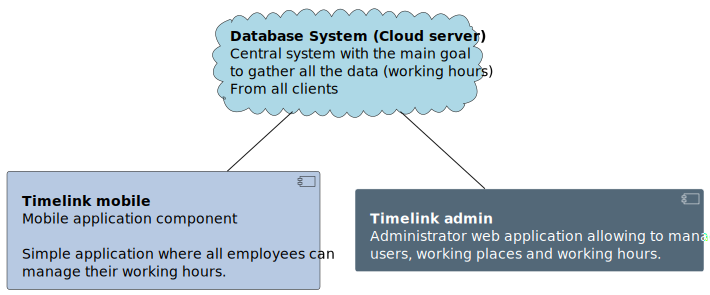
\includegraphics[width=0.75\linewidth]{./Pictures/C1_arch.png}
    \caption{C1 architecture level}
\end{figure}

\begin{figure}[hbt!]
    \centering
    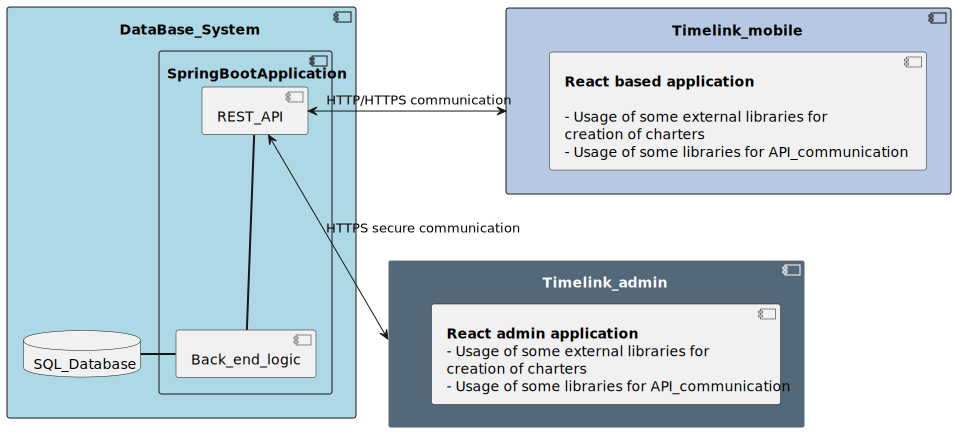
\includegraphics[width=0.75\linewidth]{./Pictures/C2_architecture.png}
    \caption{C2 architecture level}
\end{figure}

\section{Data/Network flows}

Additionally, we have also started the main communication flows for both systems, you can find sown below two data flows, one for each application.

\begin{figure}[hbt!]
    \centering
    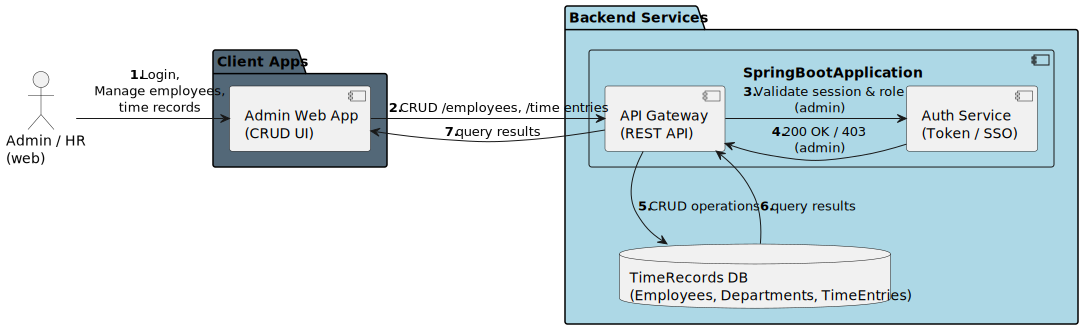
\includegraphics[width=1\linewidth]{Pictures/system_architecture.png}
    \caption{Admin app main data flow}
\end{figure}

\begin{figure}[hbt!]
    \centering
    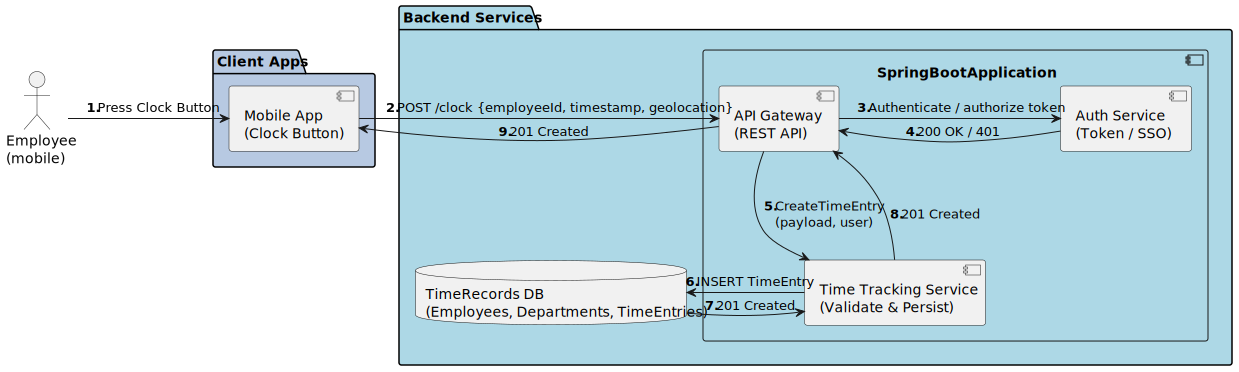
\includegraphics[width=1\linewidth]{Pictures/system_architecture_2.png}
    \caption{Mobile app main data flow}
\end{figure}

\section{UI designs}

Our team has also created some UI designs that will be used as a basis when implementing the UI of our apps.

\subsection{Timelink mobile}

\begin{figure}
    \centering
    \includegraphics[width=0.25\linewidth]{../../../SPEC/EPICS/EPIC-01/VIS/UC-US 01 - Shift Monitoring/01.jpg}
    \caption{UI related to UC-01}
\end{figure}

\begin{figure}
    \centering
    \includegraphics[width=0.25\linewidth]{../../../SPEC/EPICS/EPIC-01/VIS/UC-US 02 - Employe Shift Punch-in (Start Shift)/01.jpg}
    \includegraphics[width=0.25\linewidth]{../../../SPEC/EPICS/EPIC-01/VIS/UC-US 02 - Employe Shift Punch-in (Start Shift)/02.jpg}
    \includegraphics[width=0.25\linewidth]{../../../SPEC/EPICS/EPIC-01/VIS/UC-US 02 - Employe Shift Punch-in (Start Shift)/03.jpg}
    \caption{UI's related to UC-02}
\end{figure}

\begin{figure}
    \centering
    \includegraphics[width=0.25\linewidth]{../../../SPEC/EPICS/EPIC-01/VIS/UC-US 03 - Employe Shift Punch-out (End Shift)/01.jpg}
    \includegraphics[width=0.25\linewidth]{../../../SPEC/EPICS/EPIC-01/VIS/UC-US 03 - Employe Shift Punch-out (End Shift)/02.jpg}
    \caption{UI's related to UC-03}
\end{figure}

\begin{figure}
    \centering
    \includegraphics[width=0.25\linewidth]{../../../SPEC/EPICS/EPIC-01/VIS/UC-US 04 - Employe Reminder/01.jpg}
    \includegraphics[width=0.25\linewidth]{../../../SPEC/EPICS/EPIC-01/VIS/UC-US 04 - Employe Reminder/02.jpg}
    \includegraphics[width=0.25\linewidth]{../../../SPEC/EPICS/EPIC-01/VIS/UC-US 04 - Employe Reminder/03.jpg}
    \caption{UI's related to UC-04}
\end{figure}

\subsection{Timelink admin}

\begin{figure}
    \centering
    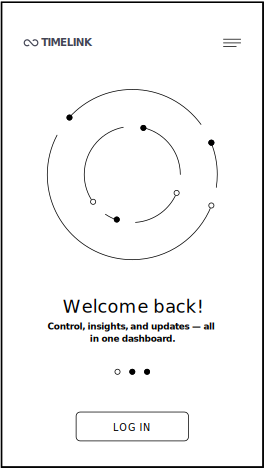
\includegraphics[width=0.25\linewidth]{./Pictures/UC-5_UC-9-1.png}
    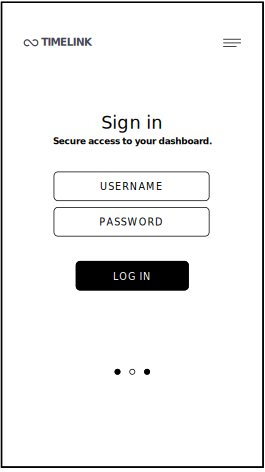
\includegraphics[width=0.25\linewidth]{./Pictures/UC-5_UC-9-2.png}
    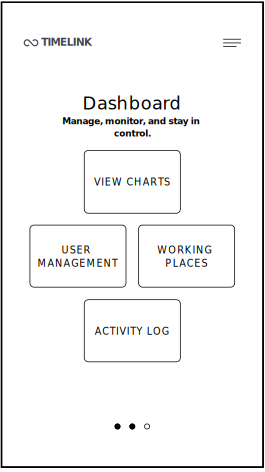
\includegraphics[width=0.25\linewidth]{./Pictures/UC-5_UC-9-3.png}
    \caption{UI's related to UC-05 and UC-09}
\end{figure}

\begin{figure}
    \centering
    \includegraphics[width=0.25\linewidth]{./Pictures/UC-6_UC-8_UC-10-1.png}
    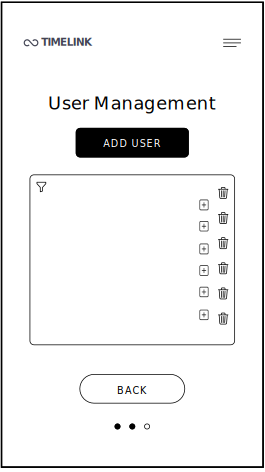
\includegraphics[width=0.25\linewidth]{./Pictures/UC-6_UC-8_UC-10-2.png}
    \caption{UI's related to UC-06 and UC-08}
\end{figure}

\begin{figure}
    \centering
    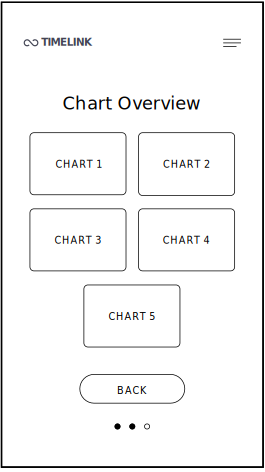
\includegraphics[width=0.25\linewidth]{./Pictures/UC-7.png}
    \caption{UI related to UC-07}
\end{figure}

\begin{figure}
    \centering
    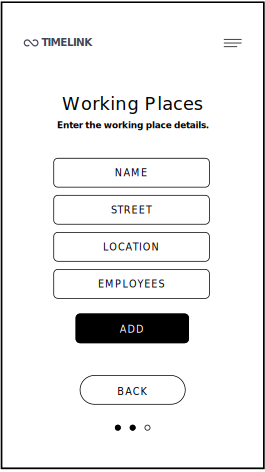
\includegraphics[width=0.25\linewidth]{./Pictures/UC-11-1.png}
    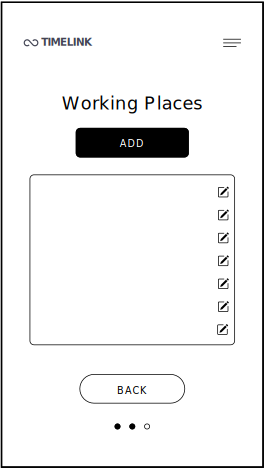
\includegraphics[width=0.25\linewidth]{./Pictures/UC-11-2.png}
    \caption{UI's related to UC-11}
\end{figure}

\begin{figure}
    \centering
    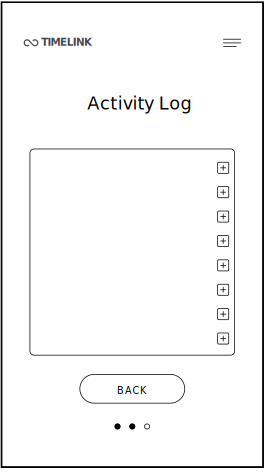
\includegraphics[width=0.25\linewidth]{Pictures/UC-12.png}
    \caption{UI related to UC-12}
\end{figure}


\chapter{Data Models}
\textbf{STILL TO DO}

\lipsum[1]

\chapter{User roles}

Currently, since our main focus for developing during the university's timeline will be to develop the mobile app (Timelink mobile), the main permissions that this user shall have are the following:

\begin{itemize}
    \item General Employee user
    \item System owner/Admin (Someone who has access to the Data server)
\end{itemize}

\section{General Employee user}

The context of this user is someone who only will be interacting with the app via the Mobile app, here are the following permissions the user shall have:

\begin{itemize}
    \item Creating new working hours under his name
    \item Change existing working hours under his name
    \item Delete existing working hours under his name
    \item Have access to his working hours in a visualization format
    \item Have access to his profile and change his personal preferences
\end{itemize}

One more detailed version will be created once the development start allowing us to identify several important points that will need to be resolved.

\section{System owner}

This user will have access to the data-server. The main interaction will be under a \texttt{PHPMyAdmin} platform (current work-around until Timelink admin will be deployed). The user shall have all the same the permissions that a General employee has but shall be able to do it for all users.
Additionally, the user shall also be able to do the following:

\begin{itemize}
    \item Create new users
    \item Delete/modify existing users
\end{itemize}

\chapter{Status report}

In this section of the document you shall find all the current information related to the the current status of the system.

\section{Current Achievements}

Currently, we have completely achieved both \texttt{Milestone 1} and \texttt{Milestone 2}.
More specifically, both specifications as well as the main design of system have been defined

\section{Current project plan}

After creating all the project specifications and starting to adding all the tasks in the project Backlog, I've quickly came to a conclusion that the current Scope will be to much for the current timeline that we have left.

To compensate this issue I've taken the decision to take the application \texttt{Timelink admin} out of development since this would possibly remove all the scope creep that we are currently suffering.

Taken this information into account, the current tasks are the following:

\begin{itemize}
    \item Development of the Data Server
    \item Development of the Mobile app
    \item Planning and execution of all mobile apps
\end{itemize}

These current tasks will start as soon as possible and will be divided under the respective people. Since the Business analyst and the PM will not have a lot to do during the time left, they will try to help the others as much as possible.

\section{Financial's}



\end{document}


